% !TeX spellcheck = gl_GL-Galician
%%%%%%%%%%%%%%%%%%%%%%%%%%%%%%%%%%%%%%%%%%%%%%%%%%%%%%%%%%%%%%%%%%%%%%%%%%%%%%%%
% Preámbulo                                                                    %
%%%%%%%%%%%%%%%%%%%%%%%%%%%%%%%%%%%%%%%%%%%%%%%%%%%%%%%%%%%%%%%%%%%%%%%%%%%%%%%%

%\documentclass[11pt,a4paper,titlepage,twoside, openright]{report}
\documentclass[11pt,a4paper,titlepage,twoside, openany]{report}

%%%%%%%%%%%%%%%%%%%%%%%%%
%% SELECCIÓN DE IDIOMA %%
%%%%%%%%%%%%%%%%%%%%%%%%%
% Descomenta la línea correspondiente al idioma de la memoria
\def\idioma{esp}  % Castellano (Español)
%\def\idioma{gal} % Galego
%\def\idioma{eng} % English


%%%%%%%%%%%%%%%%%%%%%%%%%%%%%%%%%%%%%
%% DATOS DEL PROYECTO A CONFIGURAR %%
%%%%%%%%%%%%%%%%%%%%%%%%%%%%%%%%%%%%%
\def\titulo{Memoria de Prácticas en CINFO}        % cambiar aquí el título completo
\def\alumno{Pablo Soage Rodas}                  % nombre del alumno     
\def\directorA{Julián Silveira Carnota}             % nombre del director
\def\directorB{Diego Andrade Canosa}    % descomentar aquí está línea y en la portada
                                                % para incluir uno más.
                                                % De haber más añadirlos cambiando la letra por C, D, ...
\def\departamento{Enxeñaría de Computadores}                                                                                              

%%%%%%%%%%%%%%%%%%%%%%%%%%%%%%%%%
%% CARGA DEL FICHERO DE ESTILO %%
%%%%%%%%%%%%%%%%%%%%%%%%%%%%%%%%%
\usepackage{estilo_practicas}


%%%%%%%%%%%%%%%%%%%%%%%%%%%%%%%%%%%%%%%%%
%% PAQUETES QUE PUEDEN SER DE UTILIDAD %%
%%%%%%%%%%%%%%%%%%%%%%%%%%%%%%%%%%%%%%%%%

% \usepackage{alltt}       % para campos alltt, similar a verbatim pero que respecta comandos
% \usepackage{booktabs}     % permite mejorar el aspecto de las tablas con líneas de diferente grosor para el cierre
\usepackage{enumitem}     % permite personalizar los entornos de lista
% \usepackage{eurofont}    % proporciona el comando \euro
\usepackage{float}       % permite más control de objetos flotantes (tablas y figuras)
% \usepackage{hhline}      % permite personalizar las liñas horizontales en arrays y tablas
% \usepackage{longtable}   % permite construir tablas que ocupan más de una página
% \usepackage{lscape}      % permite colocar partes del documento en orientación apaisada
% \usepackage{moreverb}    % permite personalizar o entorno verbatim
% \usepackage{multirow}    % permite crear celdas que ocupan varias filas en una tabla
% \usepackage{pdfpages}    % permite insertar ficheros PDF
% \usepackage{rotating}    % permite diferentes tipos de rotaciones para los flotantes
% \usepackage{subcaption}  % permite a inclusión de varias subfiguras en una figura
% \usepackage{tabu}        % permite tablas flexibles
% \usepackage{tabularx}    % permite tablas con columnas de anchura determinada
\usepackage{listings}
\usepackage{graphicx}
\usepackage{url}

%%%%%%%%%%%%%%%%%%%%%%%%%%%%%%%%%%%%%%%%%%%%%%%%%%%%%%%%%%%%%%%%%%%%%%%%%%%%%%%%
% CUERPO PRINCIPAL DEL DOCUMENTO                                               %
%%%%%%%%%%%%%%%%%%%%%%%%%%%%%%%%%%%%%%%%%%%%%%%%%%%%%%%%%%%%%%%%%%%%%%%%%%%%%%%%

\begin{document}


%%%%%%%%%%%%%%%%%%%%%%%%%%%%%%%%%%%%%%%%
% Preliminares do documento            %
%%%%%%%%%%%%%%%%%%%%%%%%%%%%%%%%%%%%%%%%

\begin{titlepage}
\vspace*{-35pt}
\begin{minipage}{.15\linewidth}
    \begin{flushleft}
    \hspace*{-15pt}
      %\includegraphics[scale=0.15]{04_imaxes/MUEI.png}
    \end{flushleft}
  \end{minipage}
  \hfill
  \begin{minipage}{.15\linewidth}
    \begin{flushright}     
     
\includegraphics[scale=0.06]{04_imaxes/euro_inf_seal_bachelor_light background}     
    \end{flushright} 
  \end{minipage}
 
 \vspace*{30pt}
 

\includegraphics[scale=0.30]{04_imaxes/udc}\\[10pt]
  \hspace*{18pt}\textcolor{udcpink}{{\fontencoding{T1}\fontfamily{phv}\selectfont Facultade de Informática}}\\[5pt]
  \hspace*{18pt}\textcolor{udcgray}{{\fontencoding{T1}\fontfamily{phv}\selectfont Grao en Enxeñaría Informática}}\\[5pt]
  
\textcolor{udcpink}{\titlerule[0.5mm]}\\  

  \begin{center}
    {\large PRÁCTICAS EN EMPRESA} \\[25pt]
    \begin{huge}
      \begin{spacing}{1.3}
      \vspace*{10pt}
        \bfseries \titulo
      \end{spacing}
    \end{huge}
  \end{center}
  
\textcolor{udcpink}{\titlerule[0.5mm]}\\[5pt]
  \vfill
  
  \begin{flushright}
    {\large
    \begin{tabular}{ll}
      {\bf Estudante:} & \alumno \\
      {\bf Titorización na empresa:} & \directorA \\
      {\bf Titorización académica:}     & \directorB \\  % duplicar está línea con los 
                                        % que sean necesarios cambiado la letra
                                        & \departamento
    \end{tabular}}
    
  \end{flushright}
  \rightline{A Coruña, \fecha.}
  
  
\end{titlepage}

\paginablanca

%%%%%%%%%%%%%%%%%%%%%%%%%%%%%%%%%%%%%%%%
% Preliminares do documento            %
%%%%%%%%%%%%%%%%%%%%%%%%%%%%%%%%%%%%%%%%

\pagenumbering{Roman}
\setcounter{page}{1}
\bstctlcite{IEEEexample:BSTcontrol}

\tableofcontents
\listoffigures
\listoftables
\clearpage
\paginablanca

%%%%%%%%%%%%%%%%%%%%%%%%%%%%%%%%%%%%%%%%
% Capítulos da memoria                 %
%%%%%%%%%%%%%%%%%%%%%%%%%%%%%%%%%%%%%%%%

% Numeración arábiga
\pagenumbering{arabic}
\setcounter{page}{1}

\chapter{Introducción}
\label{chap:introduccion}

\lettrine{E}{n} este primer capítulo se presentan los datos básicos de la práctica, una descripción general de su temática y los objetivos principales y secundarios de la misma.

\section{Datos de la práctica}
\label{sec:datospractica}
\begin{itemize}
    \item {\bf Empresa:} CINFO
    \item {\bf Duración:} 23 Septiembre 2024 - 2 Diciembre 2024
    \item {\bf Lugar de realización:} A Coruña
    \item {\bf Tipo:} Modalidad presencial
    \item {\bf Departamento/equipo:} Equipo de IA
    \item {\bf Cargo responsable de práctica:} IA Developer Leader
\end{itemize}

\section{Objetivos}
\label{sec:objetivos}

Las prácticas se centraron en la mejora de sistemas de visión artificial y aprendizaje automático para el reconocimiento de marcadores deportivos en tiempo real, incluyendo la configuración y optimización de herramientas existentes, así como en la investigación e implementación de sistemas de síntesis de voz (TTS).

\subsection{Objetivos generales}
\begin{enumerate}
    \item Familiarización con el flujo de trabajo de machine learning de la empresa
    \item Mejorar el sistema de detección y reconocimiento de marcadores deportivos
    \item Investigar y desarrollar sistemas de síntesis de voz para narración deportiva
    \item Contribuir al desarrollo de herramientas de automatización deportiva
\end{enumerate}

\subsection{Objetivos específicos}
\begin{enumerate}
    \item Optimizar la detección de marcadores digitales en diferentes condiciones
    \item Implementar mejoras en la interfaz de configuración de marcadores
    \item Evaluar y comparar diferentes modelos de síntesis de voz
    \item Crear datasets y realizar fine-tuning de modelos TTS
    \item Ejecutar y evaluar experimentos utilizando MLflow
    \item Documentar y mantener el código desarrollado
\end{enumerate}
\chapter{Herramientas y tecnologías}
\label{chap:tecnoloxias}

\lettrine{E}{n} este capítulo, se describen las principales herramientas y tecnologías utilizadas durante el desarrollo de las prácticas. Se detallan tanto las herramientas de desarrollo como las tecnologías de Machine Learning y visión artificial empleadas.


\section{Herramientas de desarrollo}\label{sec:tecnologias}

\subsection{Control de versiones y gestión del código}\label{subsec:git}
Durante las prácticas se utilizó Git como sistema de control de versiones, junto con GitLab para el alojamiento de repositorios. Además, se emplearon las siguientes herramientas:

\begin{itemize}
    \item \textbf{pre-commit}: Herramienta\cite{pre_commit} que automatiza verificaciones en los repositorios, asegurando la unificación del formato del código y la generación de docstrings según convenciones definidas.
    \item \textbf{GitLab CI/CD}: Sistema\cite{gitlab_ci} de integración y despliegue continuo que permite ejecutar pipelines automatizados para pruebas, construcción y despliegue de aplicaciones.
    \item \textbf{DVC (Data Version Control)}: Herramienta\cite{dvc} para el versionado de datasets y modelos de Machine Learning, asegurando la reproducibilidad y rastreabilidad de experimentos.
\end{itemize}

\subsection{Entorno de desarrollo}\label{subsec:entorno}
El desarrollo se realizó principalmente en Python, utilizando:

\begin{itemize}
    \item \textbf{Visual Studio Code}: IDE\cite{vscode} principal utilizado para la escritura, depuración y administración del código con extensiones específicas para Python.
    \item \textbf{Docker y docker-compose}: Herramientas\cite{docker} para la contenerización, facilitando la creación de entornos aislados y reproducibles para el desarrollo y la ejecución de aplicaciones.
    \item \textbf{Conda y venv}: Utilizados\cite{conda}\cite{venv} para la gestión de entornos virtuales en Python, permitiendo un manejo eficiente de dependencias.
    \item \textbf{CMake y Make}: Herramientas\cite{cmake} empleadas para la configuración y compilación de proyectos, especialmente útiles en componentes de software de bajo nivel.
\end{itemize}

\section{Tecnologías de Machine Learning y Visión Artificial}
\label{sec:ml}

\subsection{MLflow}\label{subsec:mlflow}
Se utilizó MLflow\cite{mlflow} para la gestión de experimentos de Machine Learning, permitiendo:

\begin{itemize}
    \item \textbf{Tracking de métricas y parámetros}: Registro de datos relevantes durante los entrenamientos, como la pérdida y las tasas de aprendizaje.
    \item \textbf{Versionado de modelos}: Gestión de diferentes versiones de modelos entrenados, facilitando su comparación y reutilización.
    \item \textbf{Comparación de experimentos}: Análisis detallado entre distintas ejecuciones para identificar las configuraciones más efectivas.
    \item \textbf{Reproducibilidad de resultados}: Garantiza que los experimentos sean replicables al registrar todas las configuraciones necesarias.
\end{itemize}

\begin{figure}[hp!]
  \centering
  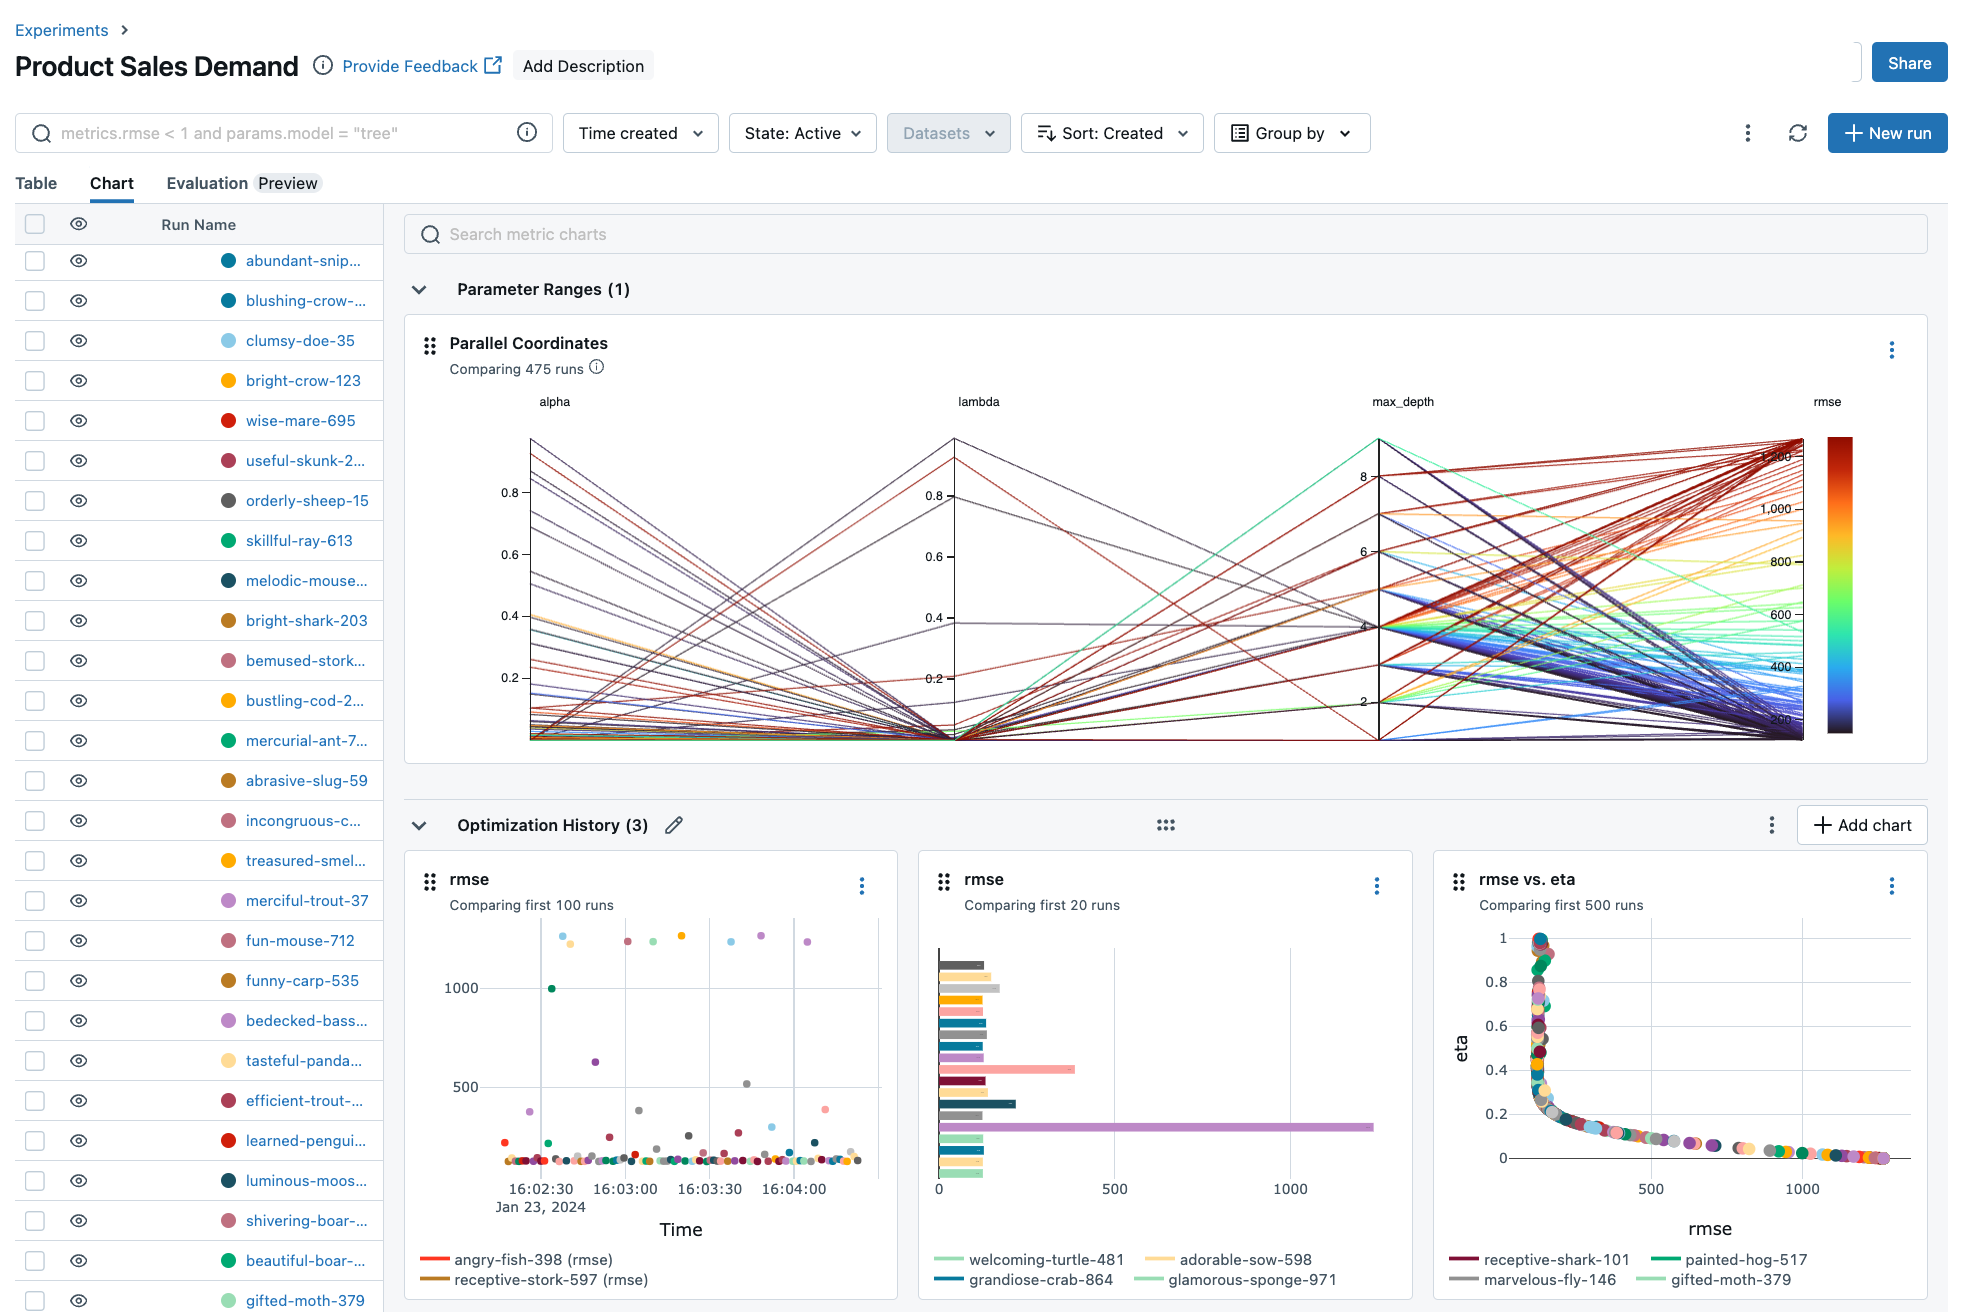
\includegraphics[width=0.8\textwidth]{04_imaxes/mlflow_example.png}
  \caption{Interfaz de gestión de experimentos en MLflow}
  \label{fig:mlflow}
\end{figure}

\subsection{CVAT}\label{subsec:cvat}
Para el etiquetado de datos se empleó CVAT\cite{cvat} (Computer Vision Annotation Tool), que permite:

\begin{itemize}
    \item \textbf{Etiquetado de videos frame a frame}: Ofrece una interfaz intuitiva para marcar objetos en cada fotograma.
    \item \textbf{Definición de bounding boxes}: Herramienta esencial para delimitar regiones de interés en imágenes o videos.
    \item \textbf{Exportación en múltiples formatos}: Compatible con una amplia variedad de formatos estándar en proyectos de visión artificial.
    \item \textbf{Trabajo colaborativo}: Facilita la asignación de tareas y la colaboración entre varios usuarios en un mismo proyecto.
\end{itemize}

\begin{figure}[hp!]
  \centering
  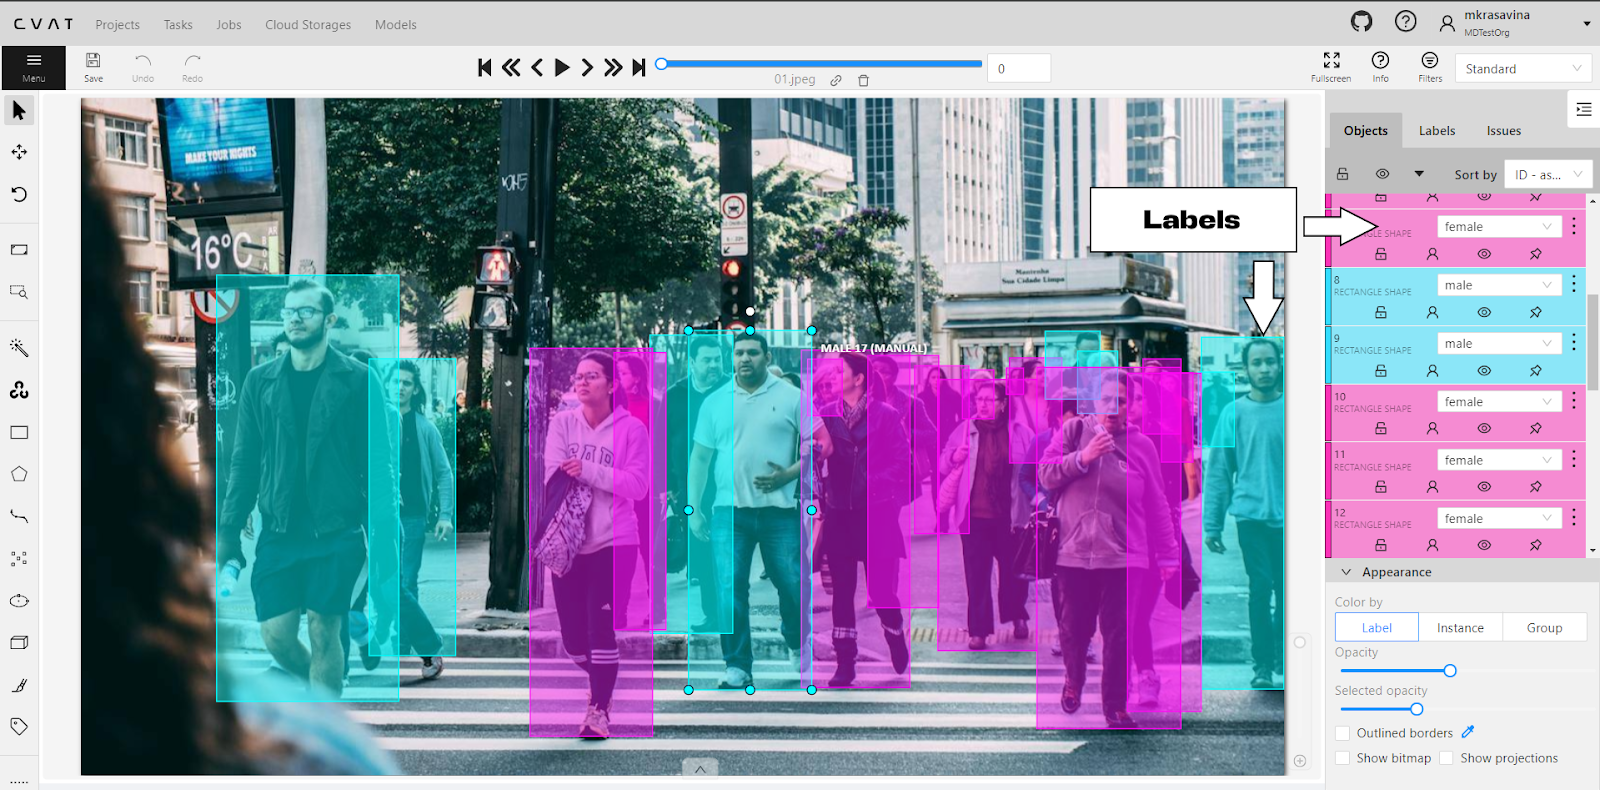
\includegraphics[width=0.8\textwidth]{04_imaxes/cvat_example.png}
  \caption{Ejemplo de etiquetado en CVAT}
  \label{fig:cvat}
\end{figure}

\section{Tecnologías de Síntesis de Voz (TTS)}
\label{sec:tts}

Durante las prácticas se evaluaron múltiples modelos de Text-to-Speech (TTS), analizando sus características y capacidades. A continuación, se presentan los modelos evaluados:

\subsection{Coqui TTS}\label{subsec:coqui}
Plataforma\cite{coqui_tts} de código abierto que incluye múltiples modelos TTS:
\begin{itemize}
    \item \textbf{XTTSv2}: Especializado en clonación de voz, permitiendo la reproducción de voces específicas con alta fidelidad.
    \item \textbf{Tacotron2 con HiFi-GAN}: Combinación\cite{tacotron2} de un modelo de texto a mel-espectrograma (Tacotron2) con un generador de audio de alta calidad (HiFi-GAN), ideal para síntesis natural.
    \item \textbf{VITS}: Modelo\cite{vits} integrado para síntesis de voz y conversión de voz a texto, que equilibra calidad y rapidez.
\end{itemize}

\subsection{IMS-Toucan}\label{subsec:ims_toucan}
Modelo\cite{ims_toucan} de síntesis desarrollado por el Instituto de Ciencias de la Computación de Stuttgart. Ofrece capacidades avanzadas de generación de voz con enfoque en la naturalidad y entonación, aunque no incluye soporte completo para clonación de voz. Dispone de cierta compatibilidad con clonación de voz pero, la voz generada, será como la voz más similar empleada en el entrenamiento. Sin embargo, esto puede mitigarse en parte mediante el fine-tunning.

\subsection{Otros modelos evaluados}\label{subsec:other_models}
Además de los anteriores, se probaron los siguientes modelos TTS:

\begin{itemize}
    \item \textbf{OpenVoice v2}: Sistema\cite{openvoice} TTS flexible y de código abierto, diseñado para personalización y soporte multilingüe.
    \item \textbf{Real-Time-Voice-Cloning}: Modelo que combina Tacotron y redes neuronales para realizar clonación de voz y síntesis de alta calidad en tiempo real.
    \item \textbf{Mozilla TTS}: Plataforma\cite{mozilla_tts} modular y extensible para la síntesis de voz, enfocada en facilitar la creación de modelos personalizados y adaptativos.
\end{itemize}

\subsection{Modelos que no soportan clonado de voz}\label{subsec:no_clonado}

A lo largo de las prácticas se evaluaron diversos modelos de Text-to-Speech que no cuentan con capacidad de clonación de voz. A continuación, se listan algunos de ellos:

\begin{itemize}
    \item \textbf{eSpeak}: Motor TTS ligero y rápido que genera síntesis de voz basada en reglas. Aunque no soporta clonado, es eficiente para dispositivos de baja capacidad.
    \item \textbf{Festival}: Sistema TTS modular y flexible que ofrece varias opciones para la generación de voces sintéticas, pero carece de funcionalidad para clonación.
    \item \textbf{Mimic1}: Derivado de Festival, Mimic1 permite una síntesis rápida con diferentes voces preconfiguradas, sin soporte para clonación de voz.
    \item \textbf{Mimic3}: Continuación de Mimic1, diseñada para síntesis offline con menor latencia y mejor calidad de audio, pero sin capacidades de clonación.
    \item \textbf{Pico TTS}: Solución compacta para la síntesis de texto a voz orientada a dispositivos móviles, sin características avanzadas como la clonación.
    \item \textbf{Flite}: Variante ligera de Festival que se utiliza en sistemas embebidos para tareas de síntesis básica de voz.
    \item \textbf{Mary TTS}: Plataforma extensible para la síntesis de voz que soporta múltiples idiomas y configuraciones, pero no incluye clonado.
    \item \textbf{Piper}: Modelo optimizado para la generación rápida de audio TTS con una calidad aceptable, aunque no soporta clonación.
    \item \textbf{FastSpeech 2}: Modelo TTS basado en arquitectura Transformer que ofrece síntesis eficiente, pero sin capacidades de clonado directo.
    \item \textbf{TransformerTTS}: Sistema TTS basado en Transformers que produce voces naturales pero no admite clonación.
    \item \textbf{Tensorflow TTS}: Conjunto de modelos TTS basados en TensorFlow que incluyen varias arquitecturas avanzadas, sin funcionalidad de clonado.
    \item \textbf{PaddleSpeech}: Biblioteca TTS de código abierto que soporta múltiples modelos, enfocada en la síntesis pero sin capacidades de clonación.
    \item \textbf{Glow Speak}: Basado en la arquitectura Glow, este modelo TTS permite una síntesis precisa pero no incluye soporte para clonado de voz.
\end{itemize}

\section{Otras herramientas}
\label{sec:otras}

\begin{itemize}
    \item \textbf{ffmpeg}: Para procesamiento de video y audio\\
        Es una solución\cite{ffmpeg} multiplataforma ampliamente utilizada para la grabación, conversión y transmisión de archivos de audio y video. En este proyecto, se empleó para tareas como el recorte de videos/audios y la conversión de formatos, lo que permitió optimizar recursos (wav >> mp3) y garantizar compatibilidad con diferentes plataformas. 
    \item \textbf{VIA} (VGG Image Annotator): Para etiquetado de imágenes\\
        Una herramienta\cite{via} ligera y sencilla para el etiquetado de imágenes. Es crucial para preparar conjuntos de datos, ya que permite definir áreas de interés en imágenes (bounding boxes, máscaras, etc.) y asignarles etiquetas personalizadas. En este proyecto, se utilizó para generar anotaciones necesarias para entrenar modelos de reconocimiento de dígitos en marcadores.
        \begin{figure}[hp!]
          \centering
          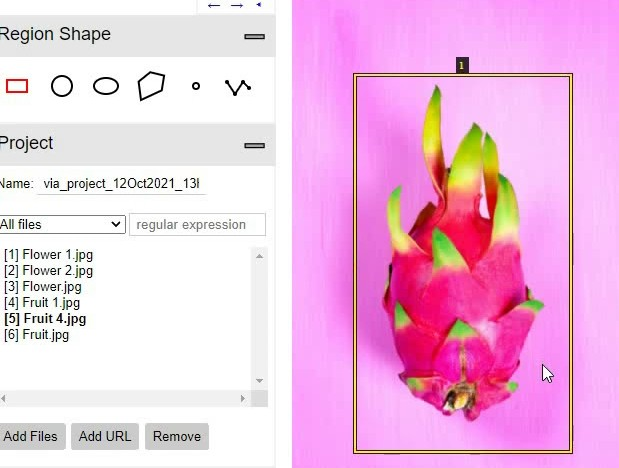
\includegraphics[width=0.8\textwidth]{04_imaxes/via_example.jpg}
          \caption{Ejemplo de etiquetado en VIA}
          \label{fig:via}
        \end{figure}
    \item \textbf{Whisper}: Para transcripción de audio\\
        Una solución desarrollada por OpenAI para la transcripción automática de audio en texto. Es una herramienta\cite{whisper} robusta que admite múltiples idiomas y ofrece transcripciones con alta precisión incluso en condiciones de ruido. Su utilización fue clave para procesar grabaciones de audio y convertirlas en datos textuales que posteriormente fueron empleados para la generación de los datasets utilizados para realizar el fine-tunning de modelos TTS.
    \item \textbf{JIRA}: Para gestión de tareas y tickets\\
        Es una plataforma\cite{jira} de gestión de tareas y seguimiento de tickets ampliamente adoptada en entornos de desarrollo de software y gestión de proyectos. La emplea la empresa para organizar y priorizar tareas, registrar incidencias, y facilitar la colaboración entre los diferentes miembros del equipo. Su capacidad para generar informes y estadísticas también contribuye al seguimiento del progreso de los proyectos y a la toma de decisiones basada en datos.\\
        En mi caso, se me asignaron trabajos o incidencias a resolver mediante dicha plataforma.
    \item \textbf{Demucs}: Para la limpieza de audios.\\
        Es un modelo\cite{demucs} de aprendizaje profundo diseñado para la separación de fuentes de audio. Permite dividir una pista de audio en componentes como voz, instrumentos y ruido de fondo, lo que facilita la limpieza y mejora de grabaciones. En este proyecto, se utilizó para aislar el contenido relevante de grabaciones de audio, eliminando ruidos no deseados y mejorando la calidad de las pistas procesadas, que serían empleadas en el para generar los datasets junto con Whisper.
     \item \textbf{OpenCV}: Para procesamiento de imágenes y visión por computadora.\\
        Es una biblioteca\cite{opencv} de código abierto ampliamente utilizada para tareas de visión artificial. Incluye funciones avanzadas para manipulación de imágenes, detección de objetos, reconocimiento facial, y análisis de video. En este proyecto, se utilizó para representar las interfaces gráficas de las utilidades, así como para interactuar con las imágenes mostradas.
    \item \textbf{Tkinter}: Para la creación de interfaces gráficas de usuario (GUI).\\
        Biblioteca estándar de Python para el desarrollo de interfaces gráficas. Proporciona herramientas para crear ventanas, botones, cuadros de texto, y otros componentes interactivos. En este proyecto, se utilizó para desarrollar una interfaz intuitiva que facilitara la interacción con el usuario, permitiendo configurar marcadores de forma sencilla, sin necesidad de realizar cambios manualmente en los json.

\end{itemize}
\chapter{Desarrollo de las prácticas}
\label{chap:desarrollo}

\lettrine{E}{n} este capítulo se describe detalladamente el trabajo realizado durante las prácticas, organizando las actividades cronológicamente y destacando los principales hitos, retos y aprendizajes.

\section{Primera etapa: Configuración y familiarización}
\label{sec:primera_etapa}

Durante la primera semana, el enfoque principal fue la configuración del entorno y la familiarización con las herramientas y flujos de trabajo de la empresa. Las actividades incluyeron:

\begin{itemize}
    \item \textbf{Presentación y configuración inicial:} Reunión con recursos humanos, entrega de equipos, claves y lectura de documentos sobre protección de datos y flujos de trabajo.
    \item \textbf{Configuración del entorno de desarrollo:} Instalación de herramientas clave como DVC, Conda, Python, Docker, Visual Studio Code con extensiones específicas (gitlens, c/c++, Python), y configuraciones para proyectos con CMake y Make.
    \item \textbf{Familiarización con las plataformas de gestión:} Estudio de herramientas internas como MLflow, CVAT y DVC, utilizadas para gestionar experimentos, etiquetado y datasets.
    \item \textbf{Primeras pruebas prácticas:} Subida y etiquetado de videos en CVAT, identificando retos como la latencia en el etiquetado de objetos móviles (ej., pelotas).
\end{itemize}

\section{Segunda etapa: Mejoras en detección de marcadores}
\label{sec:segunda_etapa}

El objetivo de esta etapa fue optimizar el sistema de detección de marcadores deportivos. Entre las actividades más relevantes destacan:

\subsection{Detección de marcadores apagados}
\label{subsec:marcadores_apagados}

Se implementaron mejoras en la detección de marcadores con bajo contraste o apagados:

\begin{itemize}
    \item \textbf{Generación de datasets específicos:} Captura y etiquetado de imágenes de marcadores en condiciones adversas.
    \item \textbf{Actualización del diccionario:} Inclusión de caracteres adicionales como espacios y símbolos necesarios para nuevos escenarios.
    \item \textbf{Reentrenamiento de modelos:} Entrenamientos iterativos con los nuevos datos para mejorar la precisión de las detecciones.
\end{itemize}

Estas mejoras se reflejaron en las métricas de Word Error Rate (WER), reduciendo el error global del 23.4\% al 18.7\% (ver Tabla \ref{tab:metricas}).

\begin{table}[h]
\centering
\begin{tabular}{|l|c|c|}
\hline
\textbf{Métrica} & \textbf{Antes} & \textbf{Después} \\
\hline
Global WER & 0.234 & 0.187 \\
\hline
\end{tabular}
\caption{Mejora en métricas de detección}
\label{tab:metricas}
\end{table}

\section{Tercera etapa: Investigación en TTS}
\label{sec:tercera_etapa}

Durante esta fase, se exploraron tecnologías de síntesis de voz, evaluando múltiples modelos y realizando pruebas exhaustivas.

\subsection{Modelos evaluados}
\label{subsec:tts_modelos}
Entre los modelos analizados, se incluyen:

\begin{itemize}
    \item \textbf{Coqui TTS:} Plataforma versátil que integra modelos como XTTSv2 (clonación de voz), Tacotron2 con HiFi-GAN (síntesis natural) y VITS.
    \item \textbf{OpenVoice v2:} Sistema TTS enfocado en personalización y soporte multilingüe.
    \item \textbf{IMS-Toucan:} Modelo que destaca por su adaptabilidad y cantidad de idiomas soportados (aunque no todos tienen la misma calidad de síntesis).
    \item \textbf{Mozilla TTS:} Herramienta extensible para la creación de modelos personalizados.
\end{itemize}

\begin{figure}[h]
    \centering
    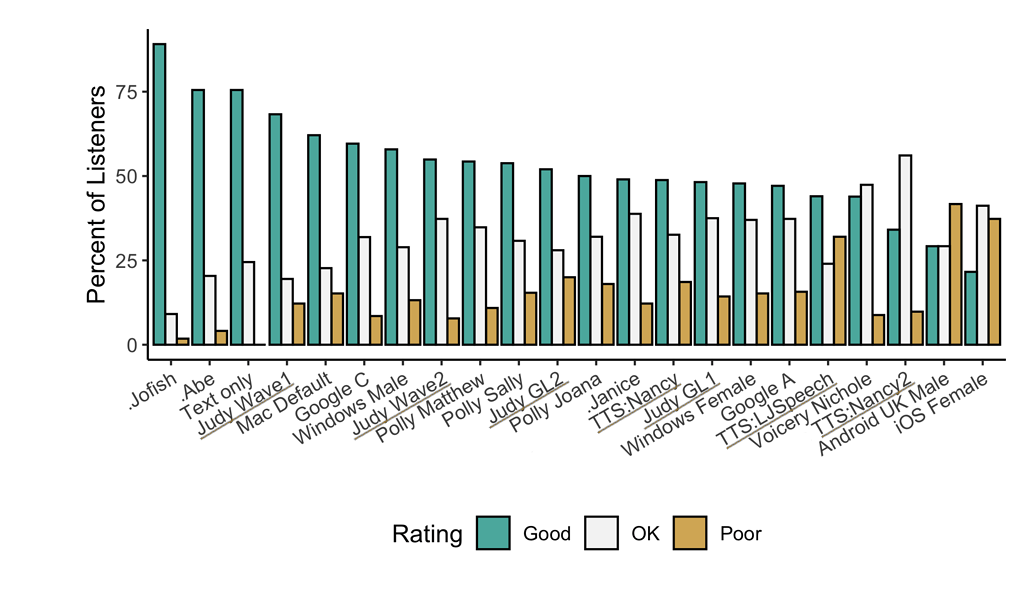
\includegraphics[width=0.8\textwidth]{04_imaxes/TTS-performance.png}
    \caption{Desempeño de modelos disponibles en Coqui TTS}
    \label{fig:tts_performance}
\end{figure}

\subsection{Fine-tuning de modelos}
\label{subsec:tts_fine_tuning}
Se realizaron ajustes finos en modelos seleccionados, siguiendo estos pasos:

\begin{itemize}
    \item \textbf{Creación de datasets:} Generación y normalización de datos de entrenamiento utilizando herramientas como Whisper y ffmpeg.
    \item \textbf{Ajustes de parámetros:} Pruebas con configuraciones avanzadas para mejorar la calidad de la síntesis.
    \item \textbf{Evaluación:} Comparación de métricas para identificar el impacto de las mejoras.
\end{itemize}

\section{Herramientas y tecnologías utilizadas}
\label{sec:herramientas}

Durante las prácticas se emplearon diversas herramientas tecnológicas, entre las que destacan:

\begin{itemize}
    \item \textbf{Control de versiones:} Git y GitLab para la gestión del código.
    \item \textbf{ML/CV:} Herramientas como MLflow, DVC y CVAT para gestionar experimentos y datasets.
    \item \textbf{Contenedores:} Docker y docker-compose para contenerización.
    \item \textbf{CI/CD:} GitLab CI y pre-commit para automatizar flujos de trabajo.
    \item \textbf{Audio/Video:} ffmpeg y Whisper para procesamiento y transcripción.
    \item \textbf{Otros:} Python, bash y tmux para tareas diversas.
\end{itemize}

\section{Retos y soluciones}
\label{sec:retos}

A lo largo de las prácticas se enfrentaron diversos desafíos, entre ellos:

\begin{itemize}
    \item \textbf{Gestión de dependencias:} Resuelto mediante el uso de entornos virtuales y Docker.
    \item \textbf{Limitaciones de hardware:} Optimización de parámetros y uso de máquinas remotas con GPUs de alta capacidad.
    \item \textbf{Problemas de inferencia:} Mejora de datasets y reentrenamiento de modelos para corregir errores específicos.
    \item \textbf{Procesos zombie:} Uso de tmux para una gestión robusta de sesiones.
\end{itemize}
\chapter{Conclusiones}
\label{chap:conclusions}

\lettrine{E}{n} este último capítulo se presenta una reflexión final sobre las prácticas realizadas, incluyendo la relación con los conocimientos adquiridos durante el grado y una valoración personal de la experiencia.

\section{Relación con la titulación}
\label{sec:titulacion}

Durante el desarrollo de las prácticas, varias asignaturas del grado han resultado especialmente útiles:

\begin{itemize}
    \item \textbf{Aprendizaje Automático}: Los conocimientos adquiridos en esta asignatura fueron fundamentales para entender y trabajar con los modelos de ML, especialmente en la parte de evaluación de métricas y entrenamiento. Las herramientas como MLflow habrían sido muy útiles para los proyectos de la asignatura.
    
    \item \textbf{Concurrencia y Paralelismo}: Los conceptos aprendidos fueron esenciales para entender y depurar problemas relacionados con threads y procesos, especialmente en el desarrollo de interfaces y en la gestión de procesos de entrenamiento.
    
    \item \textbf{Paradigmas de Programación}: La experiencia con diferentes paradigmas ayudó en la comprensión y desarrollo de código Python, especialmente en aspectos como type hints y programación funcional.
    
    \item \textbf{Visión Artificial}: Los fundamentos teóricos fueron valiosos para comprender los sistemas de visión artificial y reconocimiento de patrones.
    
    \item \textbf{Interfaces Persona Máquina}: Los conocimientos sobre diseño de interfaces facilitaron la implementación de mejoras en las herramientas de configuración.
    
    \item \textbf{Algoritmos}: La base algorítmica fue importante para optimizar procesos y mejorar la eficiencia del código.
\end{itemize}

\section{Valoración de la práctica}
\label{sec:valoracion}

Las prácticas han sido una experiencia muy enriquecedora que ha permitido:

\begin{enumerate}
    \item \textbf{Experiencia profesional real}:
    \begin{itemize}
        \item Trabajo en equipo usando metodologías ágiles
        \item Gestión de proyectos con JIRA y GitLab
        \item Participación en code reviews y merge requests
    \end{itemize}
    
    \item \textbf{Aprendizaje técnico}:
    \begin{itemize}
        \item Profundización en Python y buenas prácticas de desarrollo
        \item Uso de herramientas profesionales (Docker, Git, MLflow, DVC)
        \item Experiencia en ML/CV y procesamiento de audio
    \end{itemize}
    
    \item \textbf{Desarrollo personal}:
    \begin{itemize}
        \item Mejora en la capacidad de resolución de problemas
        \item Desarrollo de autonomía y responsabilidad
        \item Comunicación efectiva en equipo
    \end{itemize}
\end{enumerate}

\section{Lecciones aprendidas}
\label{sec:lecciones}

Entre las principales lecciones aprendidas destacan:

\begin{itemize}
    \item \textbf{Gestión de dependencias}: La importancia de mantener un control estricto de las versiones de las dependencias y el uso de entornos virtuales.
    
    \item \textbf{Documentación}: La necesidad de mantener una documentación clara y actualizada, especialmente en proyectos colaborativos.
    
    \item \textbf{Control de versiones}: La importancia de una buena gestión de ramas y commits en Git para mantener un desarrollo ordenado.
    
    \item \textbf{Optimización de recursos}: La gestión eficiente de recursos computacionales, especialmente en entrenamientos de modelos ML.
    
    \item \textbf{Testing}: La importancia de las pruebas exhaustivas antes de pasar código a producción.
\end{itemize}

%%%%%%%%%%%%%%%%%%%%%%%%%%%%%%%%%%%%%%%
% Bibliografía                        %
%%%%%%%%%%%%%%%%%%%%%%%%%%%%%%%%%%%%%%%
 \bibliographystyle{IEEEtranN}
 \bibliography{\bibconfig,03_bibliografia/bibliografia}
 %\clearpage
 
\end{document}

%%%%%%%%%%%%%%%%%%%%%%%%%%%%%%%%%%%%%%%%%%%%%%%%%%%%%%%%%%%%%%%%%%%%%%%%%%%%%%%%
